% ncse_new/p1_SystemsOfEquations/ch3_IterativeMethodsNonLinear/ex_NewtonArctan.tex
% solution:    NewtonArctan.m    ex_NewtonArctan.eps



\begin{problem}[Newton's method for \texorpdfstring{$F(x):=\arctan x$}{\emph{F(x):=arctan x} \coreproblem}]\label{prb:NewtonArctan}

  The merely local convergence of Newton's method is notorious, see\lref{sec:konv-des-newt}  and \lref{ex:loccvgnewt}.
  The failure of the convergence is often caused by the overshooting of Newton correction.
  In this problem we try to understand the observations made in \lref{ex:loccvgnewt}.

\begin{subproblem}[4]
  Find an equation satisfied by the smallest positive initial guess $x^{(0)}$ for which Newton's method does not converge when it is applied to  $F(x)=\arctan{x}$.
  \begin{hint}
  Find out when the Newton method oscillates between two values.
  \end{hint}
    \begin{hint}
  Graphical considerations may help you to find the solutions. See Figure~\ref{fig:newtonarctan}: you should find an expression for the function $g$.
  \begin{figure}
\caption{Newton iterations with $F(x)=\arctan(x)$ for the critical initial value $x^{(0)}$}
\begin{center} 
\label{fig:newtonarctan}
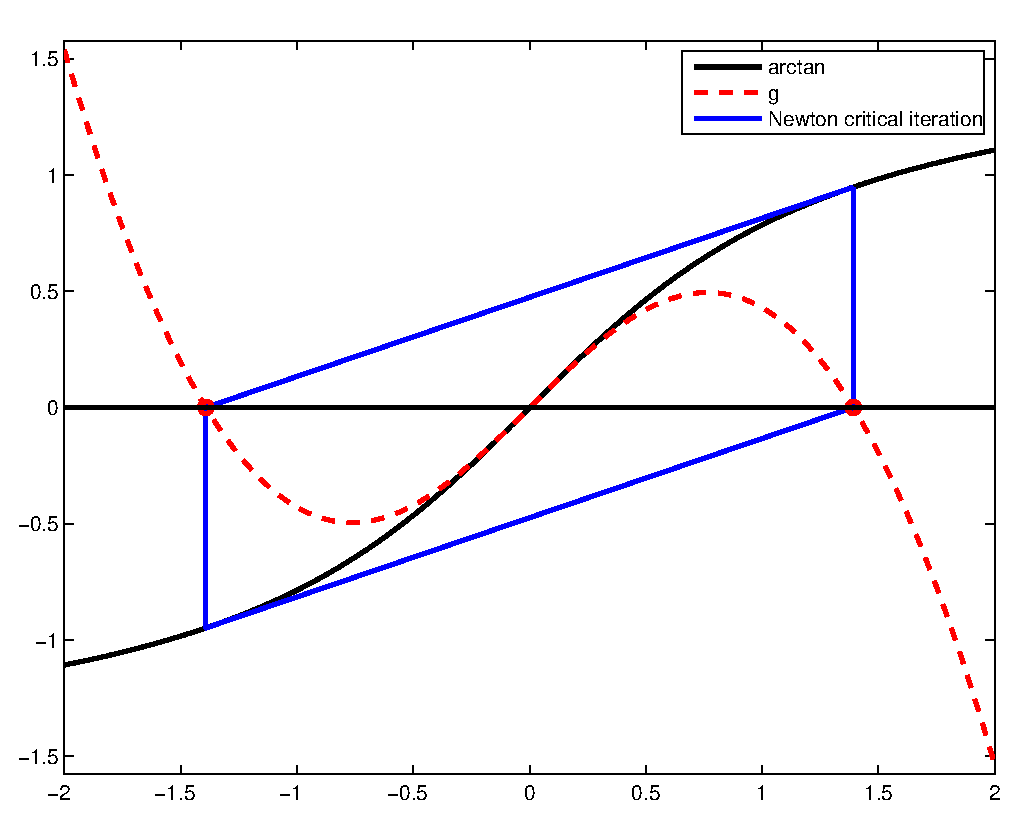
\includegraphics[width=0.6\textwidth]{\problems/ch_iterativenonlinear/PICTURES/ex_NewtonArctan.eps}
\end{center}
\end{figure}
  \end{hint}

% \Matlab's \texttt{fzero} function to compute it.  Rely on geometric considerations.


\begin{solution}The function $\arctan(x)$ is \textbf{positive, increasing and concave} for positive $x$, therefore the first iterations of Newton's method with initial points $0<x^{(0)}<y^{(0)}$ satisfy $ y^{(1)}<x^{(1)}<0$ (draw a sketch to see it).
The function is \textbf{odd}, i.e., $\arctan(-x)=-\arctan(x)$ for every $x\in\IR$, therefore the analogous holds for initial negative values ($y^{(0)}<x^{(0)}<0$ gives $0<x^{(1)}<y^{(1)}$).
Moreover, opposite initial values give opposite iterations: if $y^{(0)}=-x^{(0)}$ then $y^{(n)}=-x^{(n)}$ for every $n\in\IN$.

All these facts imply that, if $|x^{(1)}|<|x^{(0)}|$, then the absolute values of the following iterations will converge monotonically to zero.
Vice versa, if $|x^{(1)}|>|x^{(0)}|$, then  the absolute values of the Newton's iterations will diverge monotonically.
Moreover, the iterations change sign at each step, i.e., $x^{(n)}\cdot x^{(n+1)}<0$.

%Newton's method diverges for $f(x)=\arctan{x}$ if and only if $|x^{(n+1)}|\geq |x^{(n)}|$, so
It follows that the smallest positive initial guess $x^{(0)}$ for which Newton's method does not converge satisfies  $x^{(1)}= -x^{(0)}$.
This can be written as
$$x^{(1)}=x^{(0)}-\frac{f(x^{(0)})}{f'(x^{(0)})}=x^{(0)}-(1+(x^{(0)})^2)\arctan{x^{(0)}}= - x^{(0)}.$$
%The function $\arctan(x)$ is convex and negative for $x<0$ and concave and positive for $x>0$; therefore at each Newton iteration the points $x^(n)$ and $x^{(n+1)}$ have opposite signs (you can check this fact with a simple drawing).
%Thus, in the formula above we have to choose the negative sign, i.e., $x^{(1)}=-x^{(0)}$.
   Therefore, $x^{(0)}$ is  a zero of the function
    $$g(x)=2x-(1+x^2)\arctan{x} \quad \text{with} \quad g'(x)=1-2x\arctan{x}.$$
   \end{solution}
\end{subproblem}

\begin{subproblem}[2]
Use Newton's method to find an approximation of such $x^{(0)}$, and implement it with Matlab.
\cprotEnv\begin{solution}
    Newton's iteration to find the smallest positive initial guess reads
    $$x^{(n+1)}=x^{(n)}-\frac{2x^{(n)}-(1+(x^{(n)})^2)\arctan{x^{(n)}}}{1-2x\arctan{x^{(n)}}}
= \frac{ -x^{(n)}+\big(1-(x^{(n)})^2\big)\arctan x^{(n)} }{1-2x^{(n)}\arctan x^{(n)}}.$$

The implementation in Matlab is given in Listing~\ref{mc:NewtonArctan} (see also Figure~\ref{fig:newtonarctan}).

\lstinputlisting[caption={Matlab Code for \texttt{NewtonArctan.m}}, label={mc:NewtonArctan}]{\problems/ch_iterativenonlinear/MATLAB/NewtonArctan.m}





\end{solution}
\end{subproblem}

\end{problem}



% NO, WRONG:
% \textbf{Remark}: this is an example on a general phenomenon.
% Given an iterative procedure $x^{(n+1)}=\Phi(x^{(n)})$, we call a \textit{cycle} of order $k>1$ a point $x^{(0)}$ such that $x^{(k)}=x^{(0)}$ and $x^{(1)},x^{(2)},\ldots x^{(k-1)}\neq x^{(0)}$.
% A cycle of order $k$ is computed as the zero of the iterated function $g(x)=\Phi^k(x)=\Phi\circ\ldots\circ\Phi(x)$.
%
% In our case $\Phi(x)=x-F(x)/F'(x)$ is the Newton's iteration, $k=2$ and $g(x)=\Phi(\Phi(x))$.





% \subproblem\label{subprb:NewtonArctan_1}
% Consider a function $F:\IR\rightarrow \IR$ such that
% \begin{itemize}
% \item $F$ is of class $C^1(\IR)$;
% \item $F$ is odd: $F(-x) = F(x)$, $\forall\;x\in\IR$;
% \item the derivative satisfies $0<F'(x)\le 1$, $\forall\;x\in\IR$.
% \end{itemize}
% Since $F$ is strictly monotonic and odd, it follows easily that $F(x)=0$ if and only if $x=0$.
% We denote $\{x^{(k)}\}_{k=1,2,\ldots}$ a sequence of Newton iterations, i.e., $x^{(k+1)} = x^{(k)}-F(x^{(k)})/F'(x^{(k)})$, for every $k=1,2,\ldots$
%
% Prove that, for every $k\ge1$,
%  $$ \text{if}\quad0<|x^{(k+1)}|<|x^{(k)}|\quad \text{then} \quad|x^{(k+2)}|<|x^{(k+1)}|,$$
% i.e., if at the step $k$ the method is approaching the unique zero of $F$, then it will approach the zero also in the following step.
%
% \solution{We have
% \begin{align*}
%  \frac{|x^{(k+2)}|}{|x^{(k+1)}|}&
% =\frac{|x^{(k+1)}-F(x^{(k+1)})/F'(x^{(k+1)})|}{|x^{(k+1)}|}
% =\frac{|x^{(k+1)}| \cdot |1-\frac{F(x^{(k+1)})}{x^{(k+1)}}  \frac1{F'(x^{(k+1)})} | }{|x^{(k+1)}|}\\
% &= \Big|1-\underbrace{\frac{F(x^{(k+1)})}{x^{(k+1)}}}_{\in(0,1]}  \underbrace{\frac1{F'(x^{(k+1)})}}_{\in(0,1],\;\text{by }ii)} \Big|<1;
% \end{align*}
% the ratio $\frac{F(x^{(k+1)})}{x^{(k+1)}}$ is positive because an odd increasing function always has the same sign of its argument, it is smaller or equal 1 because the derivative is not larger than 1 and $F(0)=0$.
% }
%
